
\chapter{선형최소제곱 (Linear least squares)}
\label{linear}

이번 장에서 사용되는 코드는 {\tt linear.py}에 있다.
코드를 다운로드하고 작업하는 것에 대한 정보는 ~\ref{code}을 참조한다.

\section{최소제곱 적합 (Least squares fit)}

상관계수는 관계 부호와 강도를 측정하지만 기울기는 측정하지 않는다.
기울기를 측정하는 방법이 몇가지 있다; 가장 흔한 방법이 {\bf 선형최소제곱 적합 (linear least squares fit)}이다. ``선형 적합(linear fit)''은 변수 사이 관계를 모형화하는 선(line)이다.
``최소제곱 (least squares)'' 적합은 선과 데이터 사이 평균제곱오차(mean
squared error, MSE)를 최소화하는 것이다.
\index{최소제곱 적합 (least squares fit)}
\index{선형최소제곱 (linear least squares)}
\index{모형 (model)}

하나 시퀀스 {\tt ys}가 있는데, 또 다른 시퀀스 {\tt xs} 함수로 표현하고자 한다고 가정하자.
만약 {\tt xs}, {\tt ys}와 절편 {\tt inter}, 기울기 {\tt slope} 사이에 선형 관계가 있다면,
각 {\tt y[i]} 가 {\tt inter + slope * x[i]}이 될 것으로 예상된다.  
\index{잔차 (residuals)}

하지만, 상관이 완벽하지 않다면, 예측은 단지 근사(approximation)가 된다.
선에서 수직 편차(vertical deviation), 즉 {\bf 잔차(residual)}는 다음과 같다. 
\index{편차 (deviation)}

\begin{verbatim}
res = ys - (inter + slope * xs)
\end{verbatim}

잔차는 측정 오차 같은 확률 요소(random factor), 혹은 알지 못하는 비임의 요소(non-random factor) 때문일지 모른다. 예를 들어, 만약 체중을 신장 함수로 예측한다면, 미지 요소는 식습관, 운동, 신체 유형을 포함할 수 있다.

\index{기울기 (slope)}
\index{절편 (intercept)}
\index{측정 오차 (measurement error)}

만약 모수 {\tt inter}와 {\tt slope}이 잘못되면, 잔차는 더 커진다.
그래서 모수는 잔차를 최소화한다는 것이 직관적으로 의미가 있다.
\index{모수 (parameter)}

잔차 절대값, 잔차 제곱, 혹은 잔차 세제곱 최소화를 시도해볼만 하다;
하지만, 가장 흔한 선택은 제곱 잔차 합을 최소화하는 것이다. {\tt sum(res**2))}.

왜 그럴까요? 세가지 좋은 이유와 한가지 덜 중요한 이유가 있다.

\begin{itemize}

\item 제곱하게 되면 양수 잔차와 음수 잔차를 동일하게 처리하는 기능이 있는데, 보통 원하는 것이다.

\item 제곱은 큰 잔차에 더 많은 가중치를 주지만, 가장 큰 잔차가 항상 주도적인 경우에는 그렇게 많은 가중치를 주지는 않는다.

\item 만약 잔차가 상관관계가 없고 평균과 상수 (하지만 알려지지 않은 미지) 분산을 가진 정규분포라면,
최소제곱 적합은 또한 {\tt inter}와 {\tt slope}의 최대우도추정량이다. \url{https://en.wikipedia.org/wiki/Linear_regression}.  
\index{MLE}
  \index{최대우도추정량 (maximum likelihood estimator)}
\index{상관 (correlation)}

\item 제곱 잔차를 최소화하는 {\tt inter}와 {\tt slope} 값은 효과적으로 계산될 수 있다.

\end{itemize}

계산 효율성(computational efficiency)이 당면한 문제에 가장 적합한 방법을 선택하는 것보다 더 중요할 때 마지막 이유가 의미있다. 
이제는 더 이상 그럴지는 않다. 그래서, 제곱 잔차가 최소화하는 올바른 것인지만 고려한다.
\index{계산 방법 (computational methods)}
\index{제곱잔차 (squared residuals)}

예를 들어, {\tt xs}을 사용해서 {\tt ys} 값을 예측하려고 한다면,
과다 추정하는 것이 과소 추정하는 것보다 더 좋을 수도 (더 나쁠 수도) 있다.
이런 경우, 각 잔차에 대한 비용함수를 계산하고 전체 비용, {\tt sum(cost(res))}을 최소화한다.
하지만, 최소제곱 적합을 계산하는 것이 빠르고, 쉽고, 종종 충분히 만족스럽다.
\index{비용 함수 (cost function)}


\section{구현 (Implementation)}

{\tt thinkstats2}에 선형최소제곱을 시연하는 간단한 함수가 있다.
\index{LeastSquares}

\begin{verbatim}
def LeastSquares(xs, ys):
    meanx, varx = MeanVar(xs)
    meany = Mean(ys)

    slope = Cov(xs, ys, meanx, meany) / varx
    inter = meany - slope * meanx

    return inter, slope
\end{verbatim}

{\tt LeastSquares}는 시퀀스 {\tt xs}와 {\tt ys}을 인자로 받고 추정한 모수 {\tt inter}와
{\tt slope}을 반환한다. 동작방법에 관한 자세한 사항은 웹사이트 참조. \url{http://wikipedia.org/wiki/Numerical_methods_for_linear_least_squares}.
\index{모수 (parameter)}


{\tt thinkstats2}는 {\tt FitLine}를 제공하는데, {\tt inter} 와 {\tt slope}을 인자로 받아서 시퀀스 {\tt xs}에 대해서 적합선을 반환한다.
\index{FitLine}

\begin{verbatim}
def FitLine(xs, inter, slope):
    fit_xs = np.sort(xs)
    fit_ys = inter + slope * fit_xs
    return fit_xs, fit_ys
\end{verbatim}

이 함수를 사용해서 산모 연령 함수로 출생 체중에 대한 최소제곱을 계산할 수 있다.
\index{출생 체중 (birth weight)}
\index{체중 (weight)!출생 (birth)}
\index{연령 (age)}

\begin{verbatim}
    live, firsts, others = first.MakeFrames()
    live = live.dropna(subset=['agepreg', 'totalwgt_lb'])
    ages = live.agepreg
    weights = live.totalwgt_lb

    inter, slope = thinkstats2.LeastSquares(ages, weights)
    fit_xs, fit_ys = thinkstats2.FitLine(ages, inter, slope)
\end{verbatim}

추정한 절편과 기울기는 년마다 6.8 lbs, 0.017 lbs 이다.
이러 형태로 값을 해석하기는 어렵다: 절편은 산모 연령이 0 에서 신생아 기대 체중인데,
문맥상 의미가 없고, 기울기는 너무 작아서 쉽게 이해가 되지 않는다.
\index{기울기 (slope)}
\index{절편 (intercept)}
\index{dropna}
\index{NaN}


$x=0$에 절편을 제시하는 대신에, 절편을 평균에 제시하는 것이 종종 도움이 된다.
이 경우에, 평균 나이는 약 25세이고, 25세 산모에 대한 평균 아이 체중은 7.3 파운드다.
기울기는 년마다 0.27 온스(ounces) 즉, 10년마다 0.17 파운드가 된다.

\begin{figure}
% linear.py
\centerline{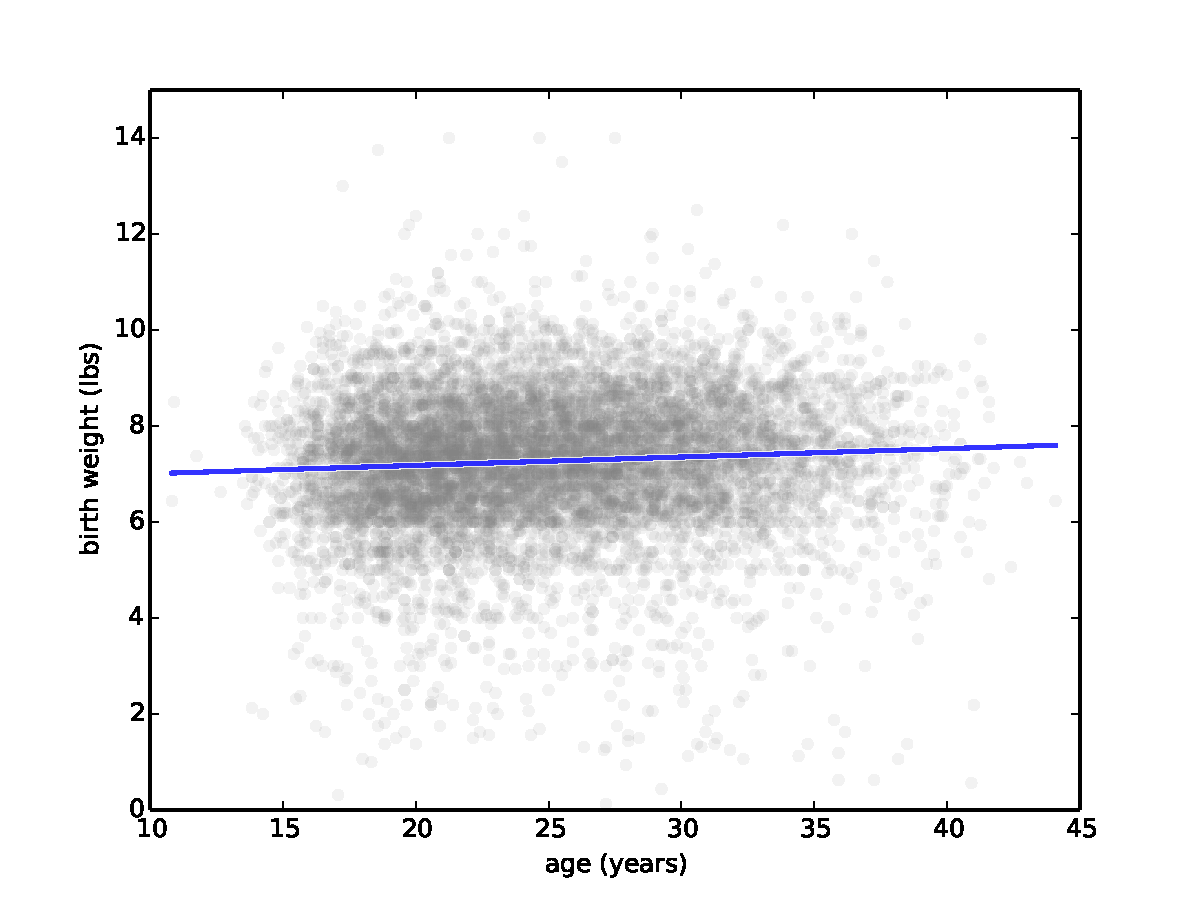
\includegraphics[height=2.5in]{figs/linear1.pdf}}
\caption{선형적합한 산모연령과 출생체중 산점도.}
\label{linear1}
\end{figure}

그림~\ref{linear1}에 적합선과 함께 출생 체중과 연령을 산점도로 보여준다.
이와 같이, 관계가 선형인지, 적합선이 관계를 나타내는 좋은 모형인지를 평가하는데, 그림을 그려보는 것은 좋은 생각이 된다. 

\index{출생 체중 (birth weight)}
\index{체중 (weight)!출생 (birth)}
\index{산점도 (scatter plot)}
\index{그림 (plot)!산점 (scatter)}
\index{모형 (model)}


\section{잔차 (Residuals)}
\label{residuals}

또다른 유용한 검정은 잔차를 플롯하여 그리는 것이다.
{\tt thinkstats2}에는 잔차를 계산하는 함수가 있다.
\index{잔차 (residuals)}

\begin{verbatim}
def Residuals(xs, ys, inter, slope):
    xs = np.asarray(xs)
    ys = np.asarray(ys)
    res = ys - (inter + slope * xs)
    return res
\end{verbatim}

{\tt Residuals}는 시퀀스 {\tt xs}와 {\tt ys}, 추정한 {\tt inter}와 {\tt slope}를 인자로 받는다. 실제값과 적합선 사이 차이를 반환한다.

\begin{figure}
% linear.py
\centerline{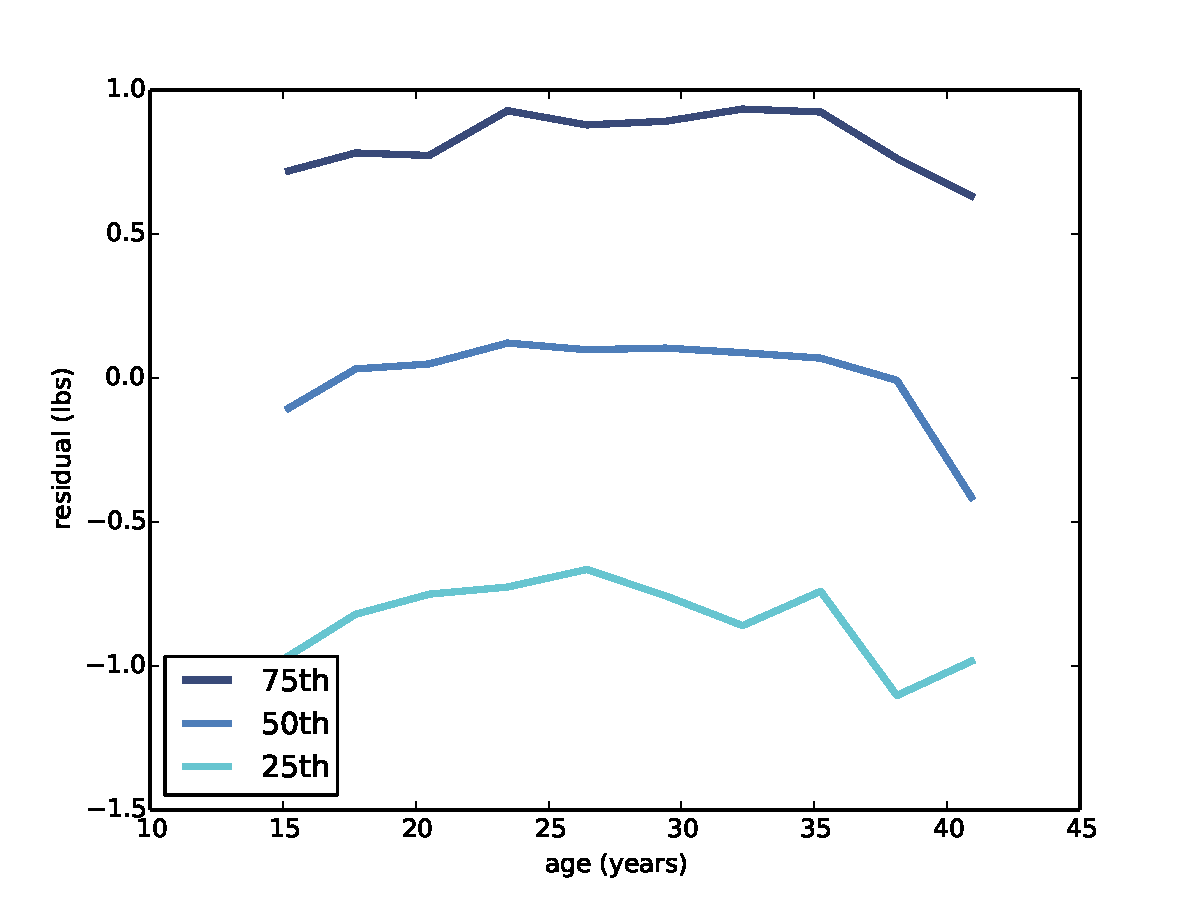
\includegraphics[height=2.5in]{figs/linear2.pdf}}
\caption{선형적합 잔차.}
\label{linear2}
\end{figure}

잔차를 시각화하기 위해서, ~\ref{characterizing} 절에서 살펴본 것과 같이, 응답자를 연령으로 묶고, 각 집단에 백분위수를 계산한다. 
그림~\ref{linear2}에 각 연령 집단에 대한 25번째, 50번째, 75번째 백분위수가 있다.
중위수는 예상한 것처럼 거의 0이고, 사분위수 범위는 약 2 파운드다. 그래서, 만약 산모 연령을 알고 있다면, 1 파운드 내에서 대략 50\% 가능성으로 아이 체중을 추측할 수 있다.
\index{시각화 (visualization)}

이상적으로 이들 직선이 평평해서 잔차가 랜덤(random)임을 나타내고, 
평행해서 잔차 분산이 모든 연령 집단에 대해서 동일하다는 것을 나타내야 한다.
사실, 직선은 평행에 가깝워서 좋다; 하지만, 약간의 곡률(curvature)이 있어서 관계가 비선형임을 나타낸다.
그럼에도 불구하고, 선형 적합은 간단한 모형으로 특정 목적에 아마도 잘 부합한다.  

\index{모형 (model)}
\index{비선형 (nonlinear)}


\section{추정 (Estimation)}
\label{regest}

모수 {\tt slope}와 {\tt inter}는 표본에 기반한 추정값이다; 다른 추정값처럼, 표집 편의, 측정 오차, 표집 오차에 휘둘리기 쉽다. 
~\ref{estimation} 장에서 논의한 것처럼, 표집 편의는 비대표 표집(non-representative sampling)에 의해서, 측정 오차는 데이터 수집과 기록 오류에 의해서, 표집 오차는 전체 모집단보다 표본을 측정하는 결과로 발생한다.
\index{표집 편의 (sampling bias)}
\index{편의 (bias)!표집 (sampling)}
\index{측정 오차 (measurement error)}
\index{표집 오차 (sampling error)}
\index{추정 (estimation)}

표집 오차를 평가하기 위해서, ``만약 이 실험을 다시 실행한다면,
추정값에 얼마나 변동성이 예상될까?''
이러한 질문에 모의시험 실험을 진행하고, 추정값에 대한 표집 분포를 계산함으로써 대답할 수 있다.

\index{표집 오차 (sampling error)}
\index{표집 분포 (sampling distribution)}

데이터를 재표본추출(resampling)하으로써 실험을 모의시험할 수 있다; 즉, 관측된 임신을 마치 전체 모집단인 것처럼 처리해서 관측된 표본에서 복원 추출 방식으로 표본을 추출한다.
\index{모의 시험 (simulation)}
\index{복원 (replacement)}

\begin{verbatim}
def SamplingDistributions(live, iters=101):
    t = []
    for _ in range(iters):
        sample = thinkstats2.ResampleRows(live)
        ages = sample.agepreg
        weights = sample.totalwgt_lb
        estimates = thinkstats2.LeastSquares(ages, weights)
        t.append(estimates)

    inters, slopes = zip(*t)
    return inters, slopes
\end{verbatim}

{\tt SamplingDistributions} 함수는 인자로 정상 출산마다 한 줄(row)로 된 데이터프레임과 모의 시험 실험 횟수, {\tt iters}를 인자로 받는다. {\tt ResampleRows}을 사용해서 관측 임신을 재표본추출한다. 이미 {\tt SampleRows}를 살펴봤는데, 데이터프레임에서 무작위(random) 행을 선택한다. {\tt thinkstats2}는 또한 {\tt ResampleRows} 기능도 제공하는데, 원본과 동일한 크기 표본을 반환한다.
\index{데이터프레임 (DataFrame)}
\index{재표본추출 (resampling)}

\begin{verbatim}
def ResampleRows(df):
    return SampleRows(df, len(df), replace=True)
\end{verbatim}

재표본추출 후에, 모의 시험 표본을 사용해서 모수를 추정한다.
결과는 시퀀스 두개다: 추정 절편과, 추정 기울기.

\index{모수 (parameter)}

표준 오차와 신뢰구간을 출력해서 표집 분포를 요약한다.
\index{표집 분포 (sampling distribution)}

\begin{verbatim}
def Summarize(estimates, actual=None):
    mean = thinkstats2.Mean(estimates)
    stderr = thinkstats2.Std(estimates, mu=actual)
    cdf = thinkstats2.Cdf(estimates)
    ci = cdf.ConfidenceInterval(90)
    print('mean, SE, CI', mean, stderr, ci)
\end{verbatim}

{\tt Summarize}는 추정값과 실제값 시퀀을 인자로 받는다. 추정값 평균, 표준 오차, 그리고, 90\% 신뢰구간을 출력한다.
\index{표준 오차 (standard error)}
\index{신뢰 구간 (confidence interval)}

절편에 대해서, 평균 추정값은 6.83, 표준오차(SE)는 0.07, 90\% 신뢰구간(CI) (6.71, 6.94)이다. 좀더 간략한 형식으로, 추정 절편 0.0174, SE 0.0028, CI (0.0126, 0.0220)가 된다. 이 신뢰구간 하한과 상한 사이에 거의 두배 차이난다. 그래서, 개략적인 추정값으로 봐야한다.

%inter 6.83039697331 6.83174035366
%SE, CI 0.0699814482068 (6.7146843084406846, 6.9447797068631871)
%slope 0.0174538514718 0.0173840926936
%SE, CI 0.00276116142884 (0.012635074392201724, 0.021975282350381781)

추정값의 표집 오차를 시각화하기 위해서, 적합선을 모두 플롯으로 그리고, 연하게 채워서 각 연령에 대해서 90\% 신뢰구간을 플롯으로 그린다. 다음에 코드가 있다.

\begin{verbatim}
def PlotConfidenceIntervals(xs, inters, slopes,
                            percent=90, **options):
    fys_seq = []
    for inter, slope in zip(inters, slopes):
        fxs, fys = thinkstats2.FitLine(xs, inter, slope)
        fys_seq.append(fys)

    p = (100 - percent) / 2
    percents = p, 100 - p
    low, high = thinkstats2.PercentileRows(fys_seq, percents)
    thinkplot.FillBetween(fxs, low, high, **options)
\end{verbatim}

{\tt xs}는 산모 연령 시퀀스다. {\tt inters}와 {\tt slopes}는 {\tt SamplingDistributions}에서 생성된 추정 모수다. {\tt percent} 인자는 플롯을 얼마의 신뢰구간으로 그릴 것인지 나타낸다.

{\tt PlotConfidenceIntervals}는 {\tt inter}와 {\tt slope} 짝에 대해 적합선을 생성하고, 결과를 시퀀스 \verb"fys_seq"에 저장한다.
그리고 나서, {\tt PercentileRows}을 사용해서 {\tt x} 각 값에 대해서 {\tt y} 상한과 하한 백분위수를 선택한다. 
90\% 신뢰구간에 대해서, 5번째와 95번째 백분위수를 선택한다. 
{\tt FillBetween}은 두 직선 사이 공간을 채우는 다각형을 그린다.
\index{thinkplot}
\index{FillBetween}

\begin{figure}
% linear.py
\centerline{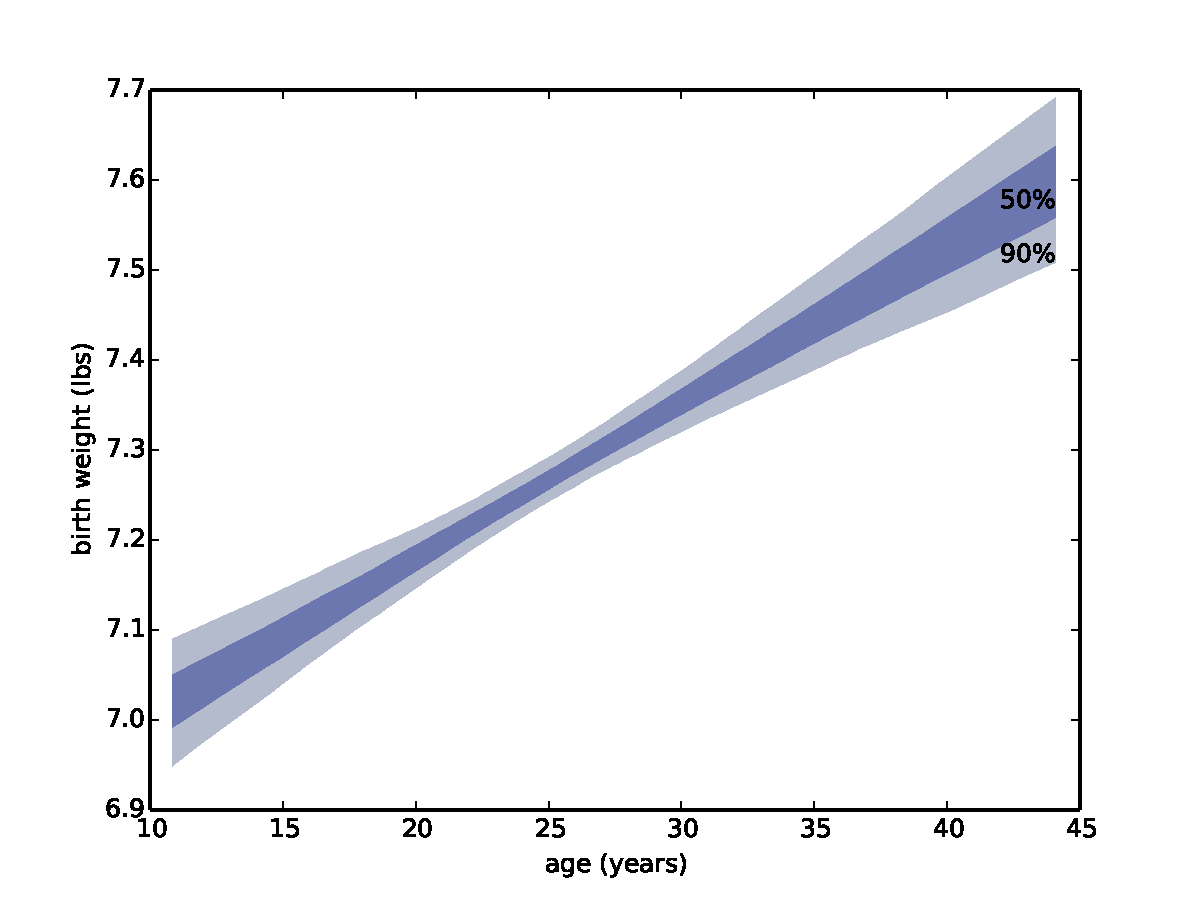
\includegraphics[height=2.5in]{figs/linear3.pdf}}
\caption{{\tt inter} 와 {\tt slope} 표집오차 때문에,
적합선에 변동성을 나타내는 신뢰구간 50\% 와 90\%.}
\label{linear3}
\end{figure}

그림~\ref{linear3}에는 산모 연령에 대한 함수로 출생 체중에 적합된 곡선에 대한 50\% 와 90\% 신뢰구간이 있다. 구역의 수직폭(vertical width)이 표집 오차에 대한 효과를 표현한다; 효과가 평균 주변 값에 대해 더 작고, 극단값에 대해 더 크다.

\section{적합도 (Goodness of fit)}
\label{goodness}
\index{적합도 (goodness of fit)}

선형 모형 품질, 즉 {\bf 적합도 (goodness of fit)}를 측정하는 방법이 몇가지 있다. 가장 간단한 방법은 잔차의 표준편차다.

\index{표준 편차 (standard deviation)}
\index{모형 (model)}

만약 예측을 위해 선형 모형을 사용한다면, {\tt Std(res)}는 예측의 제곱근 평균제곱오차(root mean squared error, RMSE)다.
예를 들어, 만약 출생 체중을 추측하는데 산모 연령을 사용한다면, 추측 RMSE는 1.40 lbs가 된다.
\index{출생 체중 (birth weight)}
\index{체중 (weight)!출생 (birth)}

만약 산모 나이를 모른 상태에서 출생 체중을 추측한다면, 
추측 RMSE는 {\tt Std(ys)}로, 1.41 lbs다.  
그래서, 이 예제에서 산모 연령을 알고 있는 것은 그다지 예측력을 향상시키지 못한다.
\index{예측 (prediction)}

적합도를 측정하는 또 다른 방식은 $R^2$로 표기하고, ``R-제곱(R-squared)''라고 부르는 {\bf 결정계수 (coefficient of determination)}다.

\index{결정계수 (coefficient of determination)}
\index{r-제곱 (r-squared)}

\begin{verbatim}
def CoefDetermination(ys, res):
    return 1 - Var(res) / Var(ys)
\end{verbatim}

{\tt Var(res)}는 모형을 사용한 추측 MSE 이고, {\tt Var(ys)}는 
모형없는 MSE 다. 그래서, 비율이 만약 모형을 사용한다면 남게되는 MSE 부분이다. $R^2$ 는 모형이 제거하는 MSE 부분이 된다.
\index{MSE}

출산 체중과 산모 나이에 대해, $R^2$ 값은 0.0047 으로, 산모 나이가 출생 체중에 있는 분산 약 0.5\%만 예측한다는 의미가 된다.

결정계수와 피어슨 상관계수 사이에 간단한 관계가 있다: $R^2 = \rho^2$.
예를 들어, 만약 $\rho$ 가 0.8 혹은 -0.8 이라면, $R^2 = 0.64$가 된다.
\index{피어슨 상관계수 (Pearson coefficient of correlation)}

$\rho$와 $R^2$가 종종 관계 강도를 정량화하는데 사용될지라도,
예측력(predictive power)에 대해서 해석하기는 쉽지 않다.
저자 견해로는, {\tt Std(res)}가 예측 품질을 가장 잘 표현한다고 본다. 특히, 만약 {\tt Std(ys)}와 연관되어 표현되면 그렇다. 

\index{결정계수 (coefficient of determination)}
\index{r-제곱 (r-squared)}

예를 들어, SAT(미국 대학 입학시험에 사용되는 표준국가시험) 타당성에 대해서 얘기할 때, 종종 사람들은 SAT 점수와 다른 지능(IQ) 측정값 사이에 상관을 얘기한다.
\index{SAT}
\index{지능 (IQ)}

한 연구에 의하면, SAT 점수와 IQ 점수 사이에 피어슨 상관은 $\rho=0.72$ 으로, 강한 상관처럼 보인다.
하지만, $R^2 = \rho^2 = 0.52$ 이여서 SAT 점수는 IQ 분산의 단지 52\%만 설명한다.

IQ 점수는 {\tt Std(ys) = 15} 로 정규화된다. 그래서, 

\begin{verbatim}
>>> var_ys = 15**2
>>> rho = 0.72
>>> r2 = rho**2
>>> var_res = (1 - r2) * var_ys
>>> std_res = math.sqrt(var_res)
10.4096
\end{verbatim}

IQ 예측하는데 SAT 점수를 사용하는 것은 RMSE를 15 점에서 10.4 점으로 줄인다. 상관계수 0.72 는 RMSE 를 줄이는데 단지 31\% 기여한다.

만약 상관계수가 감명적으로 보인다면, $R^2$이 MSE 축소에 더 나은 지표가 되고, RMSE 축소가 예측력에 대한 더 나은 지표다.

\index{결정계수 (coefficient of determination)}
\index{r-제곱 (r-squared)}
\index{예측 (prediction)}


\section{선형 모형 검정 (Testing a linear model)}

출생 체중에 대한 산모 연령 효과가 작고, 거의 예측력이 없다.
그래서, 외관 관계(apparent relationship)가 유연에 의해서 가능한 것인가?
선형적합 결과를 검정하는 방법이 몇개 있다.
\index{출생 체중 (birth weight)}
\index{체중 (weight0!출생 (birth)}
\index{모형 (model)}
\index{선형 모형 (linear model)}

한 선택옵션은 MSE에 외관 축소(apparent reduction)가 우연에 의한 것인지 검정하는 것이다. 이 경우에 검정 통계량은 $R^2$ 이고, 귀무 가설은 변수 간 관계가 없다가 된다. ~\ref{corrtest} 절에서 산모 연령과 출생 체중 간 상관을 검정했을 처럼, 귀무가설을 순열(permutation)을 통해서 모의 시험할 수 있다. 사실, $R^2 = \rho^2$, 이기 때문에, $R^2$ 단측 검정은 $\rho$ 양측 검정과 상응한다. 이미 이 검정을 수행했고, $p < 0.001$ 라는 것을 발견했다. 그래서, 산모 연령과 출생 체중 간 외관 관계는 통계적 유의성이 있다고 결론낸다.

\index{귀무 가설 (null hypothesis)}
\index{순열 (permutation)}
\index{결정계수 (coefficient of determination)}
\index{r-제곱 (r-squared)}
\index{유의성 (significant)} 
\index{통계적 유의성 (statistically significant)}

또 다른 접근법은 외관 기울기(apparent slope)가 우연에 의한 것인지 검정하는 것이다. 귀무가설은 기울기가 실제로 0 이다는 것이다; 이 경우에, 출생 체중을 평균 근처에 확률변동(random variation)으로 모형화할 수 있다. 다음에 이 모형에 대한 HypothesisTest 가 있다.
\index{HypothesisTest}
\index{모형 (model)}

\begin{verbatim}
class SlopeTest(thinkstats2.HypothesisTest):

    def TestStatistic(self, data):
        ages, weights = data
        _, slope = thinkstats2.LeastSquares(ages, weights)
        return slope

    def MakeModel(self):
        _, weights = self.data
        self.ybar = weights.mean()
        self.res = weights - self.ybar

    def RunModel(self):
        ages, _ = self.data
        weights = self.ybar + np.random.permutation(self.res)
        return ages, weights
\end{verbatim}

데이터는 연령과 체중 시퀀스로 표현된다.
검정 통계량은 {\tt LeastSquares}로 추정된 기울기다.
귀무 가설 모형은 모든 아기들의 평균 체중과 평균에 대한 편차로 표현된다.
모의 시험 데이터를 생성하기 위해서, 편차를 순열로 배치하고, 평균에 더한다.

\index{편차 (deviation)}
\index{귀무가설 (null hypothesis)}
\index{순열 (permutation)}

다음에 가설 검정을 수행하는 코드가 있다.

\begin{verbatim}
    live, firsts, others = first.MakeFrames()
    live = live.dropna(subset=['agepreg', 'totalwgt_lb'])
    ht = SlopeTest((live.agepreg, live.totalwgt_lb))
    pvalue = ht.PValue()
\end{verbatim}

p-값이 $0.001$ 보다 작다, 그래서 설사 추정된 기울기가 작지만, 우연에 의한 것 같지는 않다.

\index{p-값 (p-value)}
\index{dropna}
\index{NaN}

귀무가설을 모의 시험함으로써 p-값을 추정하는 것이 엄격하게는 맞다. 하지만, 더 간단한 대안이 있다. 이미 ~\ref{regest} 절에서 기울기 표집 분포를 계산한 것을 기억하라. 이를 위해서, 관측된 기울기가 맞다고 가정하고 재표본추출(resampling)으로 실험을 모의 시험했다.

\index{귀무가설 (null hypothesis)}

그림~\ref{linear4}에는 ~\ref{regest}절과 귀무가설 아래에서 생성된 기울기 분포에서 나온 기울기 표집 분포가 있다.
표집 분포가 추정된 기울기 약 0.017 lbs/년을 중심으로 있고, 귀무가설 아래 기울기가 약 0 을 중심으로 있다; 하지만, 그것을 제외하고 분포는 동일한다. 분포는 또한 ~\ref{CLT}절에서 살펴보게될 이유로 대칭이다. 
 
\index{대칭 (symmetric)}
\index{표집 분포 (sampling distribution)}

\begin{figure}
% linear.py
\centerline{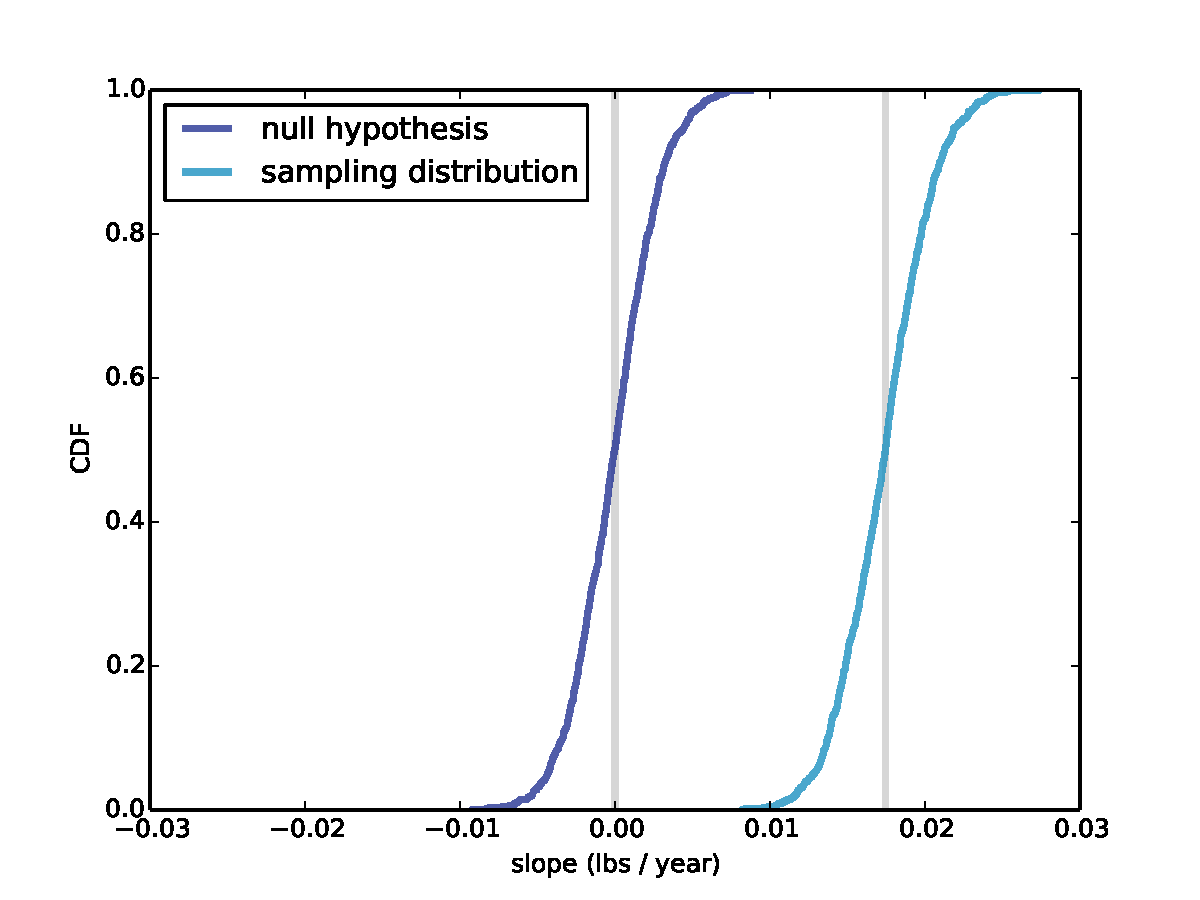
\includegraphics[height=2.5in]{figs/linear4.pdf}}
\caption{귀무가설아래 생성된 기울기 분포와 추정 기울기에 대한 표집 분포. 수직선은 0과 관측 기울기는 0.017 파운드/년.}
\label{linear4}
\end{figure}

그래서, p-값을 두 방식으로 추정할 수 있다:
\index{p-값 (p-value)}

\begin{itemize}

\item 귀무가설 아래서 기울기가 관측 기울기를 초과할 확률을 계산한다.
\index{귀무가설 (null hypothesis)}

\item 표집분포에서 기울기가 0 이하인 확률을 계산한다. (만약 추정 기울기가 음수라면, 표집 분포에서 기울기가 0을 초과하는 확률을 계산할 것이다.)

\end{itemize}

두번째 선택옵션은 더 쉬운데 이유는 어떻든 정상적으로 모수의 표집 분포를 계산하고자 하기 때문이다. 그리고 표본 크기가 작지 않고, {\em 그리고} 잔차 분포가 기울지 않았다면 좋은 근사(approximation)가 된다. 그때조차도, p-값이 정교할 필요가 없기 때문에, 대체로 만족스럽다.

\index{왜도 (skewness)}
\index{모수 (parameter)}

다음에 표집분포를 사용해서 기울기 p-값을 추정하는 코드가 있다.
\index{표집 분포 (sampling distribution)}

\begin{verbatim}
    inters, slopes = SamplingDistributions(live, iters=1001)
    slope_cdf = thinkstats2.Cdf(slopes)
    pvalue = slope_cdf[0]
\end{verbatim}

다시한번, $p < 0.001$이 나온다.  


\section{가중 재표본추출 (Weighted resampling)}
\label{weighted}

지금까지 NSFG 데이터를 마치 대표 표본인 것처럼 다루었다. 하지만, ~\ref{nsfg} 절에서 언급한 것 같이, 대표 표본은 아니다. 의도적으로 조사는 몇몇 집단을 오버샘플링(oversampling) 하는데 이유는 통계적으로 유의적인 결과를 도출할 확률을 높이기 위해서다; 즉, 이들 집단에 대해서 검정력을 향상하기 위해서다.
\index{유의성 (significant)} 
\index{통계적 유의성 (statistically significant)}

조사설계가 많은 목적에 대해서 유용하지만, 표집 과정을 고려하지 않고, 일반 모집단에 대한 값을 추정하는데 표본을 사용할 수 있다는 것을 의미하지는 않는다.

각 응답자에 대해서, NSFG 데이터는 {\tt finalwgt} 변수가 있는데, 응답자가 대표하는 일반 모집단에 속한 사람 숫자다. 이 값은 {\bf 표집 가중치 (sampling weight}, 즉 ``가중치 (weight)''라고 불린다.
\index{표집 가중치 (sampling weight)}
\index{가중치 (weight)}
\index{가중 재표본추출 (weighted resampling)}
\index{재표본추출 (resampling)!가중 (weighted)}

예제로, 만약 3억 인구를 가진 나라에서 100,000 명을 조사한다면, 각 응답자는 3,000 명을 대표한다. 만약 한 집단을 2배 오버샘플링한다면, 오버샘플링된 집단에 각 사람은 더 적은 가중치(약 1500)가 된다.

오버샘플링을 보정하기 위해서, 재표본추출(resampling)을 사용할 수 있다; 즉, 표집 가중치에 비례하는 확률을 사용해서 조사자료에서 표본을 추출한다.
그리고 나서, 추정하려고 하는 임의 정량정보에 대해서 표집 분포, 표본 오차, 신뢰구간을 생성할 수 있다. 예제로, 평균 출생 체중을 표본 가중치를 두고, 안두고 추정할 것이다.

\index{표본 오차 (standard error)}
\index{신뢰 구간 (confidence interval)}
\index{출생 체중 (birth weight)}
\index{체중 (weight)!출생 (birth)}
\index{표집 분포 (sampling distribution)}
\index{오버샘플링 (oversampling)}

~\ref{regest}절에서, {\tt ResampleRows}를 살펴봤다. 동일한 확률을 각 행에 두고 데이터프레임에서 행을 추출한다. 이제 동일한 것을 표집 가중치에 비례한 확률을 사용해서 수행할 필요가 있다. {\tt ResampleRowsWeighted}는 데이터프레임을 인자로 받고, {\tt finalwgt}에 있는 가중치에 따라 행을 재표본 추출하고, 재표본추출된 행을 포함하는 데이터프레임을 반환한다.

\index{데이터프레임 (DataFrame)}
\index{재표본추출 (resampling)}

\begin{verbatim}
def ResampleRowsWeighted(df, column='finalwgt'):
    weights = df[column]
    cdf = Cdf(dict(weights))
    indices = cdf.Sample(len(weights))
    sample = df.loc[indices]
    return sample
\end{verbatim}

{\tt weights}는 시리즈다; 시리즈를 딕셔너리로 전환하는 것은 인덱스를 가중치로 매핑한다. {\tt cdf}에서 값은 인덱스고, 확률은 가중치에 비례한다.

{\tt indices}는 행인덱스 시퀀스다; {\tt sample}은 선택된 행을 담고 있는 데이터프레임이다. 복원 표본 추출을 했기 때문에, 동일한 행이 한번이상 나올 수 있다.
\index{Cdf}
\index{복원 (replacement)}

이제, 가중치를 두고, 두지 않고 재표본추출 효과를 비교할 수 있다.
가중치를 두지 않고, 다음과 같이 표집분포를 생성한다.
\index{표집 분포 (sampling distribution)}

\begin{verbatim}
    estimates = [ResampleRows(live).totalwgt_lb.mean()
                 for _ in range(iters)]
\end{verbatim}

가중치를 두면, 다음과 같다.

\begin{verbatim}
    estimates = [ResampleRowsWeighted(live).totalwgt_lb.mean()
                 for _ in range(iters)]
\end{verbatim}

다음 표에 요약결과가 나와있다.

\begin{center}
\begin{tabular}{|l|c|c|c|}
\hline
                    &  mean birth   & standard  &  90\% CI  \\ 
                    &  weight (lbs) & error     &           \\ 
\hline
Unweighted          &  7.27  &  0.014  &  (7.24, 7.29)  \\ 
Weighted            &  7.35  &  0.014  &  (7.32, 7.37)  \\ 
\hline
\end{tabular}
\end{center}

%mean 7.26580789518
%stderr 0.0141683527792
%ci (7.2428565501217079, 7.2890814917127074)
%mean 7.34778034718
%stderr 0.0142738972319
%ci (7.3232804012858885, 7.3704916897506925)

예제애서, 가중치를 둔 효과는 적지만 무시할만하지는 않다.
가중치를 두고, 두지 않고 추정된 평균에 차이는 약 0.08 파운드, 1.3 온스다.
차이가 추정값 표준 오차(0.014 파운드)보다 실질적으로 더 크다. 함축하는 바는 차이는 우연적 요소에 의한 것은 아니라는 것이다.
\index{표준 오차 (standard error)}
\index{신뢰 구간 (confidence interval)}


\section{연습문제}

이 연습문제에 대한 해답은 \verb"chap10soln.ipynb" 파일에 나와있다.

\begin{exercise}

BRFSS에서 나온 데이터를 사용해서, log(체중) 대비 신장에 대한 선형 최소자승적합을 계산하라.
변수중 하나가 로그 변환된 이와 같은 모형에 대해서 
추정된 모수를 나타내는 가장 좋은 방식은 어떻게 될까요?
만약 누군가의 체중을 추측하려고 한다면, 신장을 아는 것이 얼마나 도움이 될까?

\index{행동위험요소 감시시스템}
\index{BRFSS}
\index{모형}

NSFG와 마찬가지로, BRFSS는 일부 집단을 과다표집(oversampling)하고 각 응답자에 대해서 표집 가중치 정보를 제공한다. BRFSS 데이터에서, 해당 가중치에 대한 변수명은 {\tt totalwt}다.
가중치를 갖는, 갖지 않는 재표집을 사용해서, BRFSS에 나온 평균 응답자 신장, 평균에 대한 표준오차, 90\% 신뢰구간을 추정하시오. 보정 가중치가 추정값에 얼마나 영향을 주는가?
\index{신뢰구간}
\index{표준오차}
\index{과다표집}
\index{표집 가중치}
\end{exercise}


\section{용어 사전}

\begin{itemize}

\item 선형적합 (linear fit): 변수 사이 관계를 모형화하려는 직선.
\index{선형적합 (linear fit)}

\item 최소제곱적합 (least squares fit): 잔차제곱합을 최소화하는 데이터셋 모형.
\index{최소제곱적합 (least squares fit)}

\item 잔차 (residual): 실제값과 모형값 편차.
\index{잔차 (residuals)}

\item 적합도 (goodness of fit): 모형이 데이터에 얼마나 잘 적합하는지에 대한 척도.
\index{적합도 (goodness of fit)}

\item 결정계수 (coefficient of determination): 적합도를 계량화하려는 통계량.
\index{결정계수 (coefficient of determination)}

\item 표집 가중치 (sampling weight): 
표본이 모집단 어느 부분을 대표하는지 나타내는데 표본 관측과 연관된 값.
\index{표집 가중치 (sampling weight)}

\end{itemize}

